\section{集合通信：分布式编程的基本积木}

在分布式训练里，最小的抽象不是“GPU”，而是 \textbf{collective operations}。它们描述的是一组 rank 之间的标准通信模式，比手工点对点通信更清晰，也更容易被 NCCL 和 PyTorch 优化。

\subsection{术语和直觉}

\begin{itemize}
    \item \textbf{World size}：参与通信的设备数量。
    \item \textbf{Rank}：某一台设备的编号，通常从 0 开始。
    \item \textbf{Collective}：所有 rank 必须配合完成的一次通信动作。
\end{itemize}

\begin{knowledgebox}{为什么“collective”这个词重要}
它强调的不是“发一条消息”，而是“大家一起完成一个固定协议”。这也是为什么分布式程序最怕漏掉一个 rank：不是少传了一条消息，而是整套协议卡住了。
\end{knowledgebox}

\begin{figure}[H]
\centering
\begin{tikzpicture}[every node/.style={font=\small, align=center}]
\node[draw, circle, minimum size=0.9cm] (r0) at (0,0) {0};
\node[draw, circle, minimum size=0.9cm] (r1) at (2,0) {1};
\node[draw, circle, minimum size=0.9cm] (r2) at (4,0) {2};
\node[draw, circle, minimum size=0.9cm] (r3) at (6,0) {3};
\draw[<->, thick] (r0) -- (r1);
\draw[<->, thick] (r1) -- (r2);
\draw[<->, thick] (r2) -- (r3);
\draw[<->, thick] (r3) -- (r0);
\node[draw, rounded corners, fill=red!8, minimum width=8cm, minimum height=1cm, below=1cm of r1] (sync) {collective 是全局协议：少一个 rank，大家都会等。};
\end{tikzpicture}
\caption{collective 不是局部动作，而是全局协议}
\end{figure}

\subsection{常见原语}

\begin{table}[H]
\centering
\small
\begin{tabular}{lll}
\toprule
\textbf{原语} & \textbf{直觉} & \textbf{用途} \\
\midrule
broadcast & 一份数据发给所有 rank & 参数同步、配置下发 \\
scatter & 一份输入切成多份分发 & 数据切片 \\
gather & 多份数据收集到一个 rank & 汇总输出 \\
reduce & 对多个值做 sum/min/max 等归约 & 梯度聚合、统计合并 \\
all-gather & 每个 rank 都拿到完整拼接结果 & 张量并行中的激活恢复 \\
reduce-scatter & 先归约，再切片分发 & all-reduce 的组成部分 \\
all-reduce & 所有 rank 最终都拿到归约结果 & DDP 梯度同步 \\
\bottomrule
\end{tabular}
\caption{常见集合通信原语}
\end{table}

\begin{importantbox}{三个容易混淆的点}
\begin{enumerate}
    \item \textbf{reduce} 不是任意函数，而通常要求可结合、可交换，例如 sum、min、max。
    \item \textbf{all} 的意思是”所有 rank 都得到结果”。
    \item \textbf{all-reduce} 常被实现为 \textbf{reduce-scatter + all-gather}，这也是很多底层优化的切入点。
\end{enumerate}
\end{importantbox}

\begin{table}[H]
\centering
\small
\resizebox{\textwidth}{!}{%
\begin{tabular}{p{2.4cm}p{3.0cm}p{3.0cm}p{2.8cm}p{4.0cm}}
\toprule
\textbf{原语} & \textbf{输入形状} & \textbf{输出形状} & \textbf{每 rank 发送量} & \textbf{典型用途} \\
\midrule
broadcast & rank 0 持有 $S$ & 所有 rank 持有 $S$ & $S$ (root 发出) & 初始化参数同步 \\
scatter & rank 0 持有 $p \times S$ & 每个 rank 持有 $S$ & $S$ (root 发出) & 数据切片分发 \\
gather & 每个 rank 持有 $S$ & rank 0 持有 $p \times S$ & $S$ (每 rank 发出) & 汇总输出、收集指标 \\
reduce & 每个 rank 持有 $S$ & rank 0 持有 $S$ & $S$ (每 rank 发出) & 梯度求和到 root \\
all-gather & 每个 rank 持有 $S$ & 所有 rank 持有 $p \times S$ & $\frac{p-1}{p} \cdot pS$ & 张量并行中恢复完整激活 \\
reduce-scatter & 每个 rank 持有 $pS$ & 每个 rank 持有 $S$ & $\frac{p-1}{p} \cdot pS$ & all-reduce 的前半段 \\
all-reduce & 每个 rank 持有 $S$ & 所有 rank 持有 $S$ & $2 \cdot \frac{p-1}{p} \cdot S$ & DDP 梯度同步（最常用） \\
\bottomrule
\end{tabular}
}
\caption{集合操作完整总结：$S$ 为单份数据大小（bytes），$p$ 为 rank 数。通信量指 ring 实现下每个 rank 的发送量。}
\end{table}

\begin{knowledgebox}{如何记忆通信量公式}
对于 ring 实现，核心因子是 $\frac{p-1}{p}$：每个 rank 在 $p-1$ 步中，每步发送 $\frac{1}{p}$ 的数据。当 $p$ 很大时，$\frac{p-1}{p} \approx 1$，也就是说每个 rank 几乎要把自己持有的全部数据发一遍。all-reduce 之所以有系数 2，是因为它包含 reduce-scatter 和 all-gather 两步，每步各传一次。
\end{knowledgebox}

\begin{figure}[H]
\centering
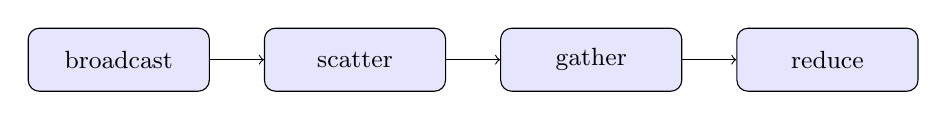
\begin{tikzpicture}[every node/.style={font=\small, align=center}]
\node[draw, rounded corners, fill=blue!10, minimum width=2.3cm, minimum height=0.8cm] (b) at (0,0) {broadcast};
\node[draw, rounded corners, fill=blue!10, minimum width=2.3cm, minimum height=0.8cm] (s) at (3.0,0) {scatter};
\node[draw, rounded corners, fill=blue!10, minimum width=2.3cm, minimum height=0.8cm] (g) at (6.0,0) {gather};
\node[draw, rounded corners, fill=blue!10, minimum width=2.3cm, minimum height=0.8cm] (r) at (9.0,0) {reduce};
\draw[->] (b) -- (s);
\draw[->] (s) -- (g);
\draw[->] (g) -- (r);
\end{tikzpicture}
\caption{广播、切分、收集与归约是最基本的通信语义}
\end{figure}

\begin{figure}[H]
\centering
\begin{tikzpicture}[every node/.style={font=\small, align=center}]
\node[draw, rounded corners, fill=yellow!10, minimum width=4.2cm, minimum height=0.9cm] (rs) at (0,0) {reduce-scatter\\先归约，再切片分发};
\node[draw, rounded corners, fill=yellow!16, minimum width=4.2cm, minimum height=0.9cm] (ag) at (5.2,0) {all-gather\\把各 rank 片段拼回来};
\node[draw, rounded corners, fill=yellow!24, minimum width=4.2cm, minimum height=0.9cm] (ar) at (10.4,0) {all-reduce\\两者组合起来};
\draw[->, thick] (rs) -- (ag);
\draw[->, thick] (ag) -- (ar);
\end{tikzpicture}
\caption{all-reduce 的常见拆法：reduce-scatter 加 all-gather}
\end{figure}

\subsection{为什么这些原语重要}

collective operations 不是“附加工具”，而是整个分布式训练的语言。你先决定模型或数据如何切分，再决定哪些切片必须通过 collective 对齐。训练策略的区别，本质上就是 \textbf{谁保留本地、谁需要交换、什么时候交换}。

\begin{warningbox}{同步点不是可选项}
如果某个 rank 少做了一次 collective，其他 rank 就会一直等。训练代码里最容易出现的 bug 之一，就是某个分支上漏掉了一个同步点，程序表面上看像“挂住了”，其实是协议不完整。
\end{warningbox}

